% PlumeProof: Round 2 slides. Team RisaavNivaran, IIT Bombay. Agentic AI Hackathon 2026, Ulster University.
% Build: tectonic plumeproof_round2.tex   (XeTeX; fonts fetched by tectonic)
% Every engine/evaluation number comes from figures/numbers.tex (generated by figures/src/gen_macros.py).
\PassOptionsToPackage{table}{xcolor}
\documentclass[aspectratio=169,10pt]{beamer}
\usepackage{fontspec}
\setsansfont{FiraSans}[Extension=.otf, UprightFont=*-Regular, BoldFont=*-SemiBold, ItalicFont=*-Italic, BoldItalicFont=*-SemiBoldItalic]
\setmonofont{FiraMono}[Extension=.otf, UprightFont=*-Regular, BoldFont=*-Bold]
\usepackage{graphicx,booktabs,tikz,amsmath,xcolor,array,tabularx}
\usepackage{unicode-math}
\setmathfont{FiraMath-Regular.otf}
\usefonttheme{professionalfonts}
\usetikzlibrary{arrows.meta,positioning,shapes.geometric,calc,fit}
\newcommand{\rupee}{₹}
% AUTO-GENERATED by src/gen_macros.py from the engine's computed numbers. Do not edit by hand.
\newcommand{\nHprior}{1.44}
\newcommand{\nHfault}{1.16}
\newcommand{\nLambda}{\rupee{}1,000}
\newcommand{\nPriorW}{50}
\newcommand{\nPriorG}{35}
\newcommand{\nPriorF}{15}
\newcommand{\nPfault}{0.43}
\newcommand{\nPostW}{6}
\newcommand{\nPostG}{65}
\newcommand{\nPostF}{29}
\newcommand{\nNoFaultW}{84}
\newcommand{\nPreLow}{1,302}
\newcommand{\nPreHigh}{2,170}
\newcommand{\nPostLow}{460}
\newcommand{\nPostHigh}{760}
\newcommand{\nThreshold}{760}
\newcommand{\nSensStab}{100}
\newcommand{\nSensTau}{0.955}
\newcommand{\nSensDraws}{200}
\newcommand{\nSensFC}{0}
\newcommand{\nSensInsp}{2.36}
\newcommand{\nSeed}{2026}
\newcommand{\nNscen}{25}
\newcommand{\nEigRec}{0.50}
\newcommand{\nCostRec}{\rupee{}2,000}
\newcommand{\nCostKRec}{\rupee{}2k}
\newcommand{\nDaysRec}{1}
\newcommand{\nGainRec}{2.50}
\newcommand{\nRankRec}{1}
\newcommand{\nEigOgi}{0.41}
\newcommand{\nCostOgi}{\rupee{}25,000}
\newcommand{\nCostKOgi}{\rupee{}25k}
\newcommand{\nDaysOgi}{2}
\newcommand{\nGainOgi}{0.17}
\newcommand{\nRankOgi}{2}
\newcommand{\nEigGnd}{0.91}
\newcommand{\nCostGnd}{\rupee{}60,000}
\newcommand{\nCostKGnd}{\rupee{}60k}
\newcommand{\nDaysGnd}{5}
\newcommand{\nGainGnd}{0.15}
\newcommand{\nRankGnd}{3}
\newcommand{\nEigSat}{0.00}
\newcommand{\nCostSat}{\rupee{}0}
\newcommand{\nCostKSat}{\rupee{}0}
\newcommand{\nDaysSat}{30}
\newcommand{\nGainSat}{--}
\newcommand{\nRankSat}{4}
\newcommand{\nFCA}{25/25}
\newcommand{\nResA}{6}
\newcommand{\nAttrA}{0\%}
\newcommand{\nSrcInspA}{0.00}
\newcommand{\nInspA}{0.00}
\newcommand{\nCostAPol}{\rupee{}0}
\newcommand{\nStakeA}{30}
\newcommand{\nTraceA}{0\%}
\newcommand{\nCloseA}{44.0}
\newcommand{\nFCB}{25/25}
\newcommand{\nResB}{15}
\newcommand{\nAttrB}{84\%}
\newcommand{\nSrcInspB}{1.80}
\newcommand{\nInspB}{3.00}
\newcommand{\nCostBPol}{\rupee{}136,667}
\newcommand{\nStakeB}{7}
\newcommand{\nTraceB}{82.8\%}
\newcommand{\nCloseB}{37.4}
\newcommand{\nFCC}{0/25}
\newcommand{\nResC}{25}
\newcommand{\nAttrC}{100\%}
\newcommand{\nSrcInspC}{0.72}
\newcommand{\nInspC}{3.00}
\newcommand{\nCostCPol}{\rupee{}128,000}
\newcommand{\nStakeC}{1}
\newcommand{\nTraceC}{100\%}
\newcommand{\nCloseC}{46.7}
\newcommand{\nFCX}{0/25}
\newcommand{\nResX}{25}
\newcommand{\nAttrX}{100\%}
\newcommand{\nSrcInspX}{0.84}
\newcommand{\nInspX}{3.24}
\newcommand{\nCostXPol}{\rupee{}127,400}
\newcommand{\nStakeX}{1}
\newcommand{\nTraceX}{100\%}
\newcommand{\nCloseX}{78.8}

\graphicspath{{figures/}}

% ---------- Theme: white, one teal accent, slate greys ----------
\definecolor{teal}{HTML}{0D9488}
\definecolor{tealL}{HTML}{CCFBF1}
\definecolor{ink}{HTML}{0F172A}
\definecolor{slate}{HTML}{64748B}
\definecolor{slateL}{HTML}{E2E8F0}
\definecolor{slateBG}{HTML}{F8FAFC}
\definecolor{alert}{HTML}{DC2626}
\definecolor{okgreen}{HTML}{16A34A}
\setbeamertemplate{navigation symbols}{}
\setbeamercolor{background canvas}{bg=white}
\setbeamercolor{normal text}{fg=ink}
\setbeamercolor{structure}{fg=teal}
\setbeamercolor{alerted text}{fg=alert}
\setbeamerfont{frametitle}{size=\Large,series=\bfseries}
\setbeamerfont{framesubtitle}{size=\small}
\setbeamertemplate{frametitle}{%
  \vspace*{0.3cm}\hspace*{-0.05cm}{\color{ink}\usebeamerfont{frametitle}\insertframetitle}%
  \ifx\insertframesubtitle\empty\else\\[0.02cm]{\color{slate}\small\insertframesubtitle}\fi
  \par\vspace*{-0.05cm}{\color{teal}\rule{1.2cm}{2pt}}\vspace*{-0.1cm}}
\setbeamertemplate{footline}{%
  \leavevmode\hbox to\paperwidth{\hspace*{0.45cm}{\color{slate}\scriptsize Team RisaavNivaran\ \ ·\ \ Agentic AI Hackathon 2026\ \ ·\ \ Ulster University}\hfill
  {\color{teal}\scriptsize\bfseries\insertframenumber}\hspace*{0.45cm}}\vspace*{0.25cm}}
\setbeamertemplate{itemize item}{\color{teal}\raisebox{0.15ex}{\small$\blacktriangleright$}}
\setbeamertemplate{itemize subitem}{\color{slate}--}
\setbeamersize{text margin left=0.6cm,text margin right=0.6cm}
\setlength{\parskip}{0pt}

\newcommand{\lbl}[2]{{\setlength{\fboxsep}{1.5pt}\colorbox{#1}{\color{white}\tiny\bfseries\,#2\,}}}
\newcommand{\REAL}{\lbl{teal}{REAL DATA}}
\newcommand{\SIM}{{\setlength{\fboxsep}{1.2pt}\fcolorbox{slate}{white}{\color{slate}\tiny\bfseries\,SIMULATED\,}}}
\newcommand{\bignum}[2]{\begin{minipage}[t]{\linewidth}\centering{\color{teal}\fontsize{30}{32}\selectfont\bfseries #1}\\[0.12cm]{\small #2}\end{minipage}}
\newcommand{\card}[2]{\begin{tikzpicture}\node[draw=slateL,fill=slateBG,rounded corners=4pt,inner sep=7pt,text width=#1,align=left]{#2};\end{tikzpicture}}
\newcommand{\shot}[2]{{\setlength{\fboxsep}{0pt}\color{slateL}\fbox{\includegraphics[#1]{#2}}}}
\newcommand{\src}[1]{{\color{slate}\tiny #1}}

\begin{document}

% =============================== 1. TITLE ===============================
\begin{frame}[t]
\vspace*{0.9cm}
\begin{columns}[T]
\begin{column}{0.47\textwidth}
{\color{teal}\small\bfseries AGENTIC AI HACKATHON 2026 · ROUND 2}\\[0.3cm]
{\fontsize{34}{36}\selectfont\bfseries PlumeProof}\\[0.25cm]
{\large From satellite methane alerts\\to \textbf{verified} mitigation}\\[0.5cm]
{\color{teal}\rule{1.2cm}{2pt}}\\[0.3cm]
{\small\textbf{Team RisaavNivaran}, IIT Bombay}\\[0.1cm]
{\small Bipra Bhanu Mohanty (lead) · Mandar Deshmukh}\\[0.1cm]
{\small\color{slate} 21–22 November 2026 · Ulster University}
\end{column}
\begin{column}{0.53\textwidth}
\vspace*{0.1cm}
\shot{width=0.985\linewidth}{landing.png}\\[0.15cm]
{\scriptsize\color{slate} A persistent case agent: it plans investigations, asks humans to approve, and refuses to close a case without independent evidence.}
\end{column}
\end{columns}
\end{frame}

% =============================== 2. VIDEO ===============================
\begin{frame}{PlumeProof in 60 seconds}
\vspace*{0.1cm}
\begin{columns}[c]
\begin{column}{0.62\textwidth}

\begin{tikzpicture}
\node[fill=ink,rounded corners=6pt,minimum width=9.0cm,minimum height=5.1cm](v){};
\node[circle,fill=teal,minimum size=1.5cm] at (v.center){};
\fill[white] ($(v.center)+(-0.22,0.35)$)--($(v.center)+(-0.22,-0.35)$)--($(v.center)+(0.38,0)$)--cycle;
\node[white,font=\small\bfseries,below=0.95cm of v.center]{Play video: \texttt{plumeproof\_60s.mp4}};
\node[slate,font=\scriptsize,above=0.15cm of v.south]{[ placeholder: video file opens from the desktop ]};
\end{tikzpicture}
\end{column}
\begin{column}{0.36\textwidth}
\small
\textbf{What you will see}
\begin{itemize}\setlength\itemsep{3pt}
\item Real plumes at Kanjur landfill, Mumbai
\item Agent ranks investigations by information per rupee
\item Operator claims a fix: \textbf{closure rejected}
\item Independent measurement: \textbf{verified}
\item New plume 14 months later: \textbf{case reopened}
\end{itemize}
\end{column}
\end{columns}
\end{frame}

% =============================== 3. PROBLEM ===============================
\begin{frame}{Detection is solved. Follow-through is not.}
\framesubtitle{The UN alert system (MARS) finds leaks from space, but few alerts lead to a verified fix}
\vspace*{0.2cm}
\begin{columns}[T]
\begin{column}{0.32\textwidth}\bignum{5,000+}{MARS alerts issued\\in 33 countries [1]}\end{column}
\begin{column}{0.32\textwidth}\bignum{13\%}{of alerts get a response\\(investigated and reported back) [1]}\end{column}
\begin{column}{0.32\textwidth}\bignum{80\%}{UN target response rate\\by 2030 [1]}\end{column}
\end{columns}
\vspace*{0.4cm}
\begin{columns}[T]
\begin{column}{0.5\textwidth}
\small
\begin{itemize}\setlength\itemsep{4pt}
\item Methane causes about \textbf{30\%} of today's warming and is about \textbf{80$\times$} more potent than CO$_2$ over 20 years [1, 7].
\item 1,015 AI-based notifications led to verified permanent mitigation at only \textbf{6} persistent emitters [5].
\end{itemize}
\end{column}
\begin{column}{0.46\textwidth}
\card{6.3cm}{\small\textbf{The gap:} after an alert, nobody owns the case. Who is responsible? What to check first? Was the fix real? Did the leak come back?\\[0.1cm]
{\color{slate}\scriptsize UNEP: satellite data alone cannot confirm mitigation [4].}}
\end{column}
\end{columns}
\end{frame}

% =============================== 4. KANJUR ===============================
\begin{frame}{Test case: Kanjur landfill, Mumbai \ \REAL}
\framesubtitle{Named among the world's three largest methane sources in a UN analysis [3]}
\begin{columns}[T]
\begin{column}{0.52\textwidth}
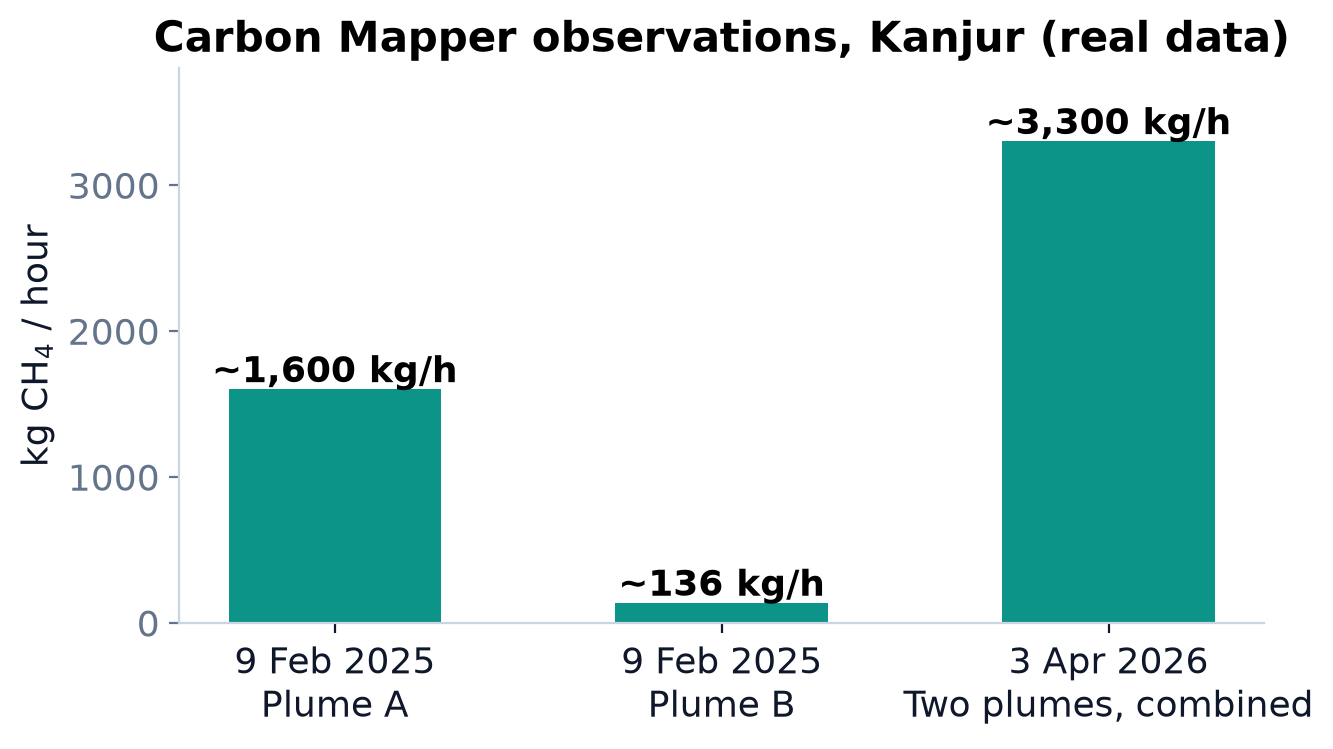
\includegraphics[width=\linewidth]{chart_kanjur.png}\\[-0.05cm]
\src{Carbon Mapper [2]. Separate satellite acquisitions under different conditions, not a continuous trend.}
\end{column}
\begin{column}{0.45\textwidth}
\small
\textbf{Why it is hard}
\begin{itemize}\setlength\itemsep{4pt}
\item Three possible sources on one site: \textbf{exposed waste surface}, \textbf{gas-collection wells and pipes}, \textbf{flare station}.
\item Odour complaints fell after odour control, but that does \emph{not} show methane fell [2].
\item The plume came back in 2026 at about 3,300 kg/h.
\end{itemize}
\vspace*{0.15cm}
\card{5.9cm}{\scriptsize\textbf{Real:} plume rates and dates. \textbf{Simulated:} operator replies, inspectors, records, repair claim, follow-up measurement. Every screen labels which is which.}
\end{column}
\end{columns}
\end{frame}

% =============================== 5. SOLUTION ===============================
\begin{frame}{What PlumeProof does}
\framesubtitle{An alert goes in. A verified, auditable outcome comes out. Humans approve every critical step.}
\vspace*{0.15cm}
\centering
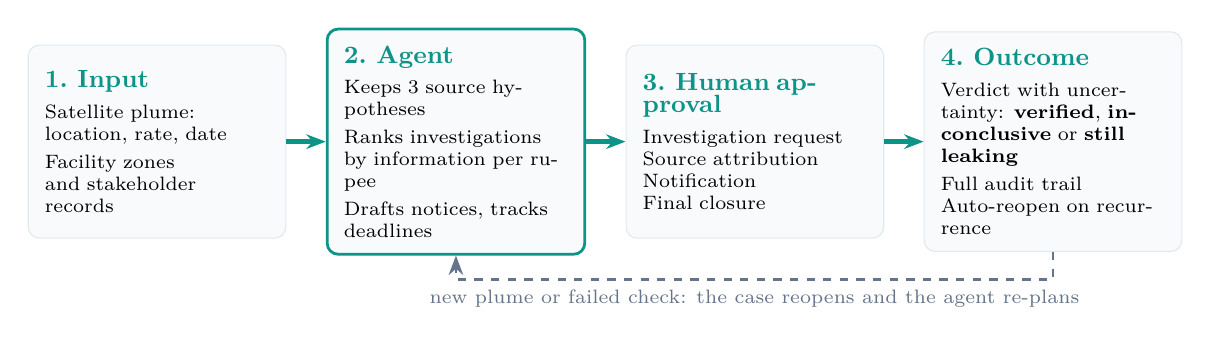
\begin{tikzpicture}[box/.style={draw=slateL,fill=slateBG,rounded corners=4pt,text width=2.85cm,minimum height=2.45cm,align=left,inner sep=6pt,font=\scriptsize},
  hd/.style={font=\small\bfseries,text=teal},arr/.style={-{Stealth[length=7pt]},line width=1.6pt,teal}]
\node[box](i){{\color{teal}\small\bfseries 1. Input}\\[3pt]Satellite plume:\\ location, rate, date\\[2pt] Facility zones\\ and stakeholder records};
\node[box,right=0.5cm of i,draw=teal,line width=1pt](a){{\color{teal}\small\bfseries 2. Agent}\\[3pt]Keeps 3 source hypotheses\\[2pt] Ranks investigations by information per rupee\\[2pt] Drafts notices, tracks deadlines};
\node[box,right=0.5cm of a](h){{\color{teal}\small\bfseries 3. Human approval}\\[3pt]Investigation request\\ Source attribution\\ Notification\\ Final closure};
\node[box,right=0.5cm of h](o){{\color{teal}\small\bfseries 4. Outcome}\\[3pt]Verdict with uncertainty: \textbf{verified}, \textbf{inconclusive} or \textbf{still leaking}\\[2pt] Full audit trail\\ Auto-reopen on recurrence};
\draw[arr](i)--(a); \draw[arr](a)--(h); \draw[arr](h)--(o);
\draw[arr,slate,line width=1pt,dashed] (o.south) -- ++(0,-0.35) -| node[pos=0.25,below,font=\scriptsize,text=slate]{new plume or failed check: the case reopens and the agent re-plans} (a.south);
\end{tikzpicture}
\vspace*{0.45cm}
\begin{columns}[T]
\begin{column}{0.95\textwidth}
\footnotesize\textbf{End users:}\ \
\textbf{regulators} (e.g.\ state pollution control board) ·
\textbf{municipal authorities} that own the site ·
\textbf{landfill / facility operators} ·
\textbf{UN IMEO MARS} national focal points
\end{column}
\end{columns}
\end{frame}

% =============================== 6. WHY AGENTIC ===============================
\begin{frame}{Why this needs an agent, not a checklist}
\framesubtitle{A case lasts months. Evidence arrives late, resources drop out and claims need checking.}
\renewcommand{\arraystretch}{1.12}
\footnotesize
\begin{tabularx}{\linewidth}{>{\bfseries}p{3.3cm} X X}
\toprule
& {\color{slate}Fixed checklist} & {\color{teal}PlumeProof agent}\\
\midrule
Memory & One pass, then done & Persistent case state for months; full audit log\\
Reasoning & Same steps, same order & Bayes' rule updates beliefs after every result\\
Planning & Fixed sequence & Picks the next action by expected information gain\\
Adapting & Stalls if a step fails & Re-plans when an inspector or record is unavailable\\
Closure & Closes on the operator's claim & Closes only on an independent measurement\\
After closure & Nothing & Watches new satellite data; reopens on recurrence\\
\bottomrule
\end{tabularx}
\vspace*{0.15cm}

\scriptsize\color{slate}\sloppy
Tools: \texttt{query\_observations}, \texttt{overlay\_facility\_zones}, \texttt{rank\_actions}, \texttt{draft\_notice}, \texttt{track\_deadline}, \texttt{evaluate\_measurement}.
Maths, rankings, verdicts and state changes are deterministic, tested code. The optional LLM only drafts text.
\end{frame}

% =============================== 7. NOVELTY 1: EIG ===============================
\begin{frame}{Novelty 1: investigate where information is cheapest}
\framesubtitle{Expected information gain (EIG): how many bits of uncertainty about the source an action removes}
\begin{columns}[T]
\begin{column}{0.40\textwidth}
\footnotesize
\vspace*{-0.2cm}
\[\mathrm{EIG}(a)=H(P)-\sum_{y}P(y\mid a)\,H\big(P(\cdot\mid y,a)\big)\]
\[\mathrm{score}(a)=\frac{\mathrm{EIG}(a)}{\mathrm{cost}(a)+\lambda\cdot\mathrm{days}(a)}\]
\vspace*{-0.1cm}
\begin{itemize}\setlength\itemsep{3pt}
\item Prior: waste \nPriorW\%, gas \nPriorG\%, flare \nPriorF\% $\Rightarrow$ $H=\nHprior$ bits
\item $\lambda$ = \nLambda{} per day (cost of delay)
\item Records show a fault $\Rightarrow$ gas collection \nPostG\%, waste \nPostW\% (Bayes' rule)
\end{itemize}
\end{column}
\begin{column}{0.58\textwidth}
\renewcommand{\arraystretch}{1.2}
\scriptsize
\begin{tabular}{@{}l r r r r@{}}
\toprule
Action & EIG (bits) & Cost & Days & {\color{teal}Bits / \rupee{}10k}\\
\midrule
\rowcolor{tealL}\textbf{Records request} & \nEigRec & \nCostRec & \nDaysRec & \textbf{\nGainRec}\\
Gas-imaging survey & \nEigOgi & \nCostOgi & \nDaysOgi & \nGainOgi\\
Ground survey & \textbf{\nEigGnd} & \nCostGnd & \nDaysGnd & \nGainGnd\\
Wait for satellite & \nEigSat & \nCostSat & \nDaysSat & \nGainSat\\
\bottomrule
\end{tabular}\\[0.25cm]
\card{7.6cm}{\scriptsize The ground survey tells us the most (\nEigGnd{} bits) but costs \nCostKGnd. The records request gives \nEigRec{} bits for \nCostKRec, so it ranks \textbf{first}. A new satellite pass says nothing about \emph{which} source: 0 bits.}
\end{column}
\end{columns}
\end{frame}

% =============================== 8. NOVELTY 2: CLOSURE ===============================
\begin{frame}{Novelty 2: a claim is not evidence}
\framesubtitle{Evidence-gated closure: the state machine has no path from ``repair reported'' to ``verified''}
\begin{columns}[T]
\begin{column}{0.53\textwidth}
\vspace*{0.2cm}
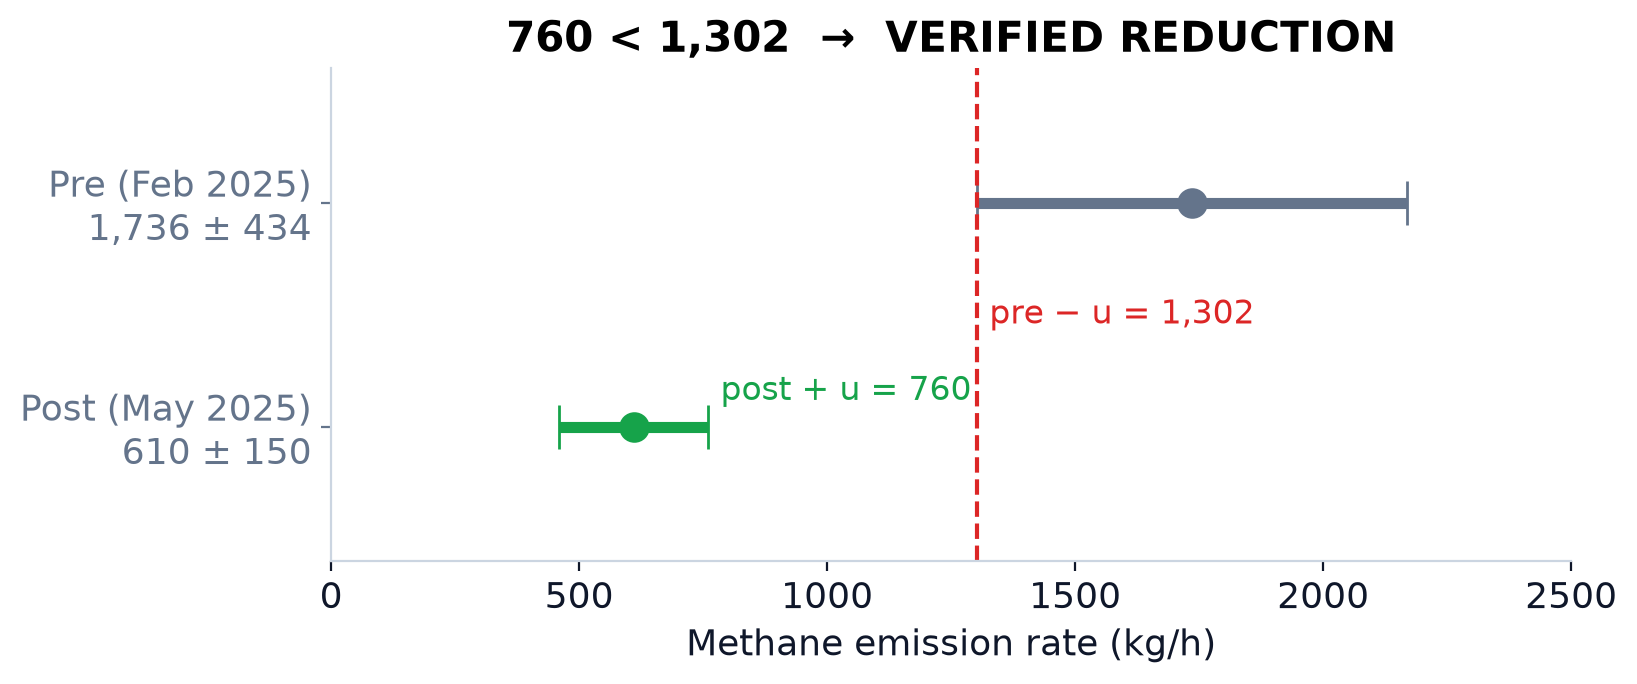
\includegraphics[width=\linewidth]{chart_verification.png}\\[-0.05cm]
\src{Pre: real 9 Feb 2025 rate, $\pm$25\% uncertainty (assumption). Post: simulated independent measurement.}
\end{column}
\begin{column}{0.44\textwidth}
\footnotesize
\card{5.8cm}{\textbf{Verified reduction} only if\\[2pt]
\centering $\text{post}+u_\text{post} < \text{pre}-u_\text{pre}$\\[2pt]
\raggedright\scriptsize from an \textbf{independent} measurement under comparable conditions.}
\vspace*{0.15cm}
\begin{itemize}\setlength\itemsep{3pt}
\item Operator's claim only $\Rightarrow$ {\color{alert}\textbf{closure rejected}}
\item Measurements disagree $\Rightarrow$ \textbf{inconclusive}, measure again
\item Upper bound $<$ lower bound $\Rightarrow$ {\color{okgreen}\textbf{verified}}, a human approves closure
\item Later plume above \nThreshold{} kg/h $\Rightarrow$ \textbf{reopened}
\end{itemize}
\end{column}
\end{columns}
\end{frame}

% =============================== 9. ARCHITECTURE ===============================
\begin{frame}{Architecture}
\framesubtitle{A deterministic core with the LLM only at the edges: with the LLM off, everything still works}
\vspace*{0.3cm}
\centering
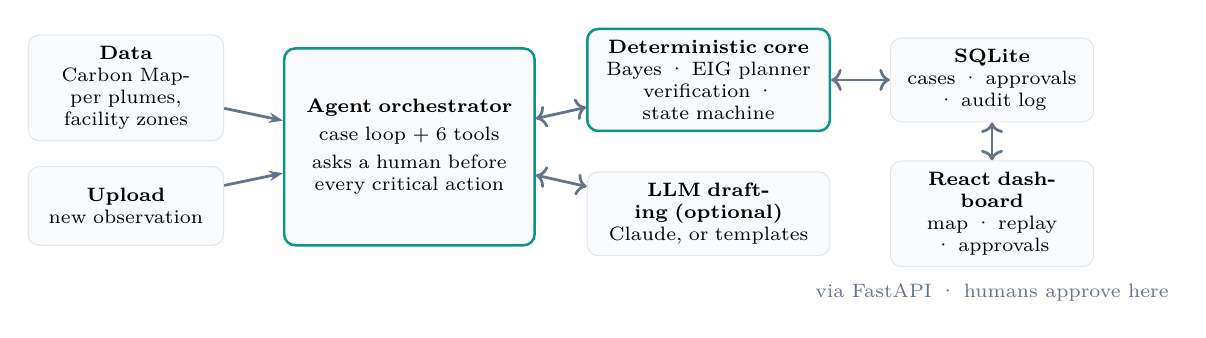
\begin{tikzpicture}[b/.style={draw=slateL,fill=slateBG,rounded corners=4pt,align=center,font=\scriptsize,inner sep=4pt,minimum height=1.0cm},
  t/.style={b,draw=teal,line width=0.9pt},arr/.style={-{Stealth[length=5pt]},line width=1pt,slate}]
\node[b,text width=2.2cm](data) at (0,0.75){\textbf{Data}\\Carbon Mapper plumes, facility zones};
\node[b,text width=2.2cm](up) at (0,-0.75){\textbf{Upload}\\new observation};
\node[t,text width=2.9cm,minimum height=2.5cm](ag) at (3.6,0){\textbf{Agent orchestrator}\\[2pt]case loop + 6 tools\\[2pt]asks a human before every critical action};
\node[t,text width=2.8cm](core) at (7.4,0.85){\textbf{Deterministic core}\\Bayes · EIG planner\\verification · state machine};
\node[b,text width=2.8cm](llm) at (7.4,-0.85){\textbf{LLM drafting (optional)}\\Claude, or templates};
\node[b,text width=2.3cm](db) at (11.0,0.85){\textbf{SQLite}\\cases · approvals · audit log};
\node[b,text width=2.3cm](ui) at (11.0,-0.85){\textbf{React dashboard}\\map · replay · approvals};
\draw[arr](data)--(ag); \draw[arr](up)--(ag);
\draw[arr,<->](ag)--(core); \draw[arr,<->](ag)--(llm);
\draw[arr,<->](core)--(db); \draw[arr,<->](db)--(ui);
\node[font=\scriptsize,text=slate,below=0.08cm of ui]{via FastAPI · humans approve here};
\end{tikzpicture}
\vspace*{0.45cm}

\scriptsize
\begin{tabular}{@{}>{\bfseries}l l @{\hspace{0.6cm}} >{\bfseries}l l@{}}
Backend & Python 3.12, FastAPI, Pydantic, SQLite & Frontend & React, Leaflet map, Recharts, offline snapshot\\[2pt]
Ship & one Docker container on Render & Tests & 128 backend tests + 3 browser end-to-end tests\\
\end{tabular}
\end{frame}

% =============================== 10. LIVE DEMO ===============================
\begin{frame}{MVP: live demo}
\framesubtitle{11-step replay of the Kanjur case. Every click on \textbf{Approve} is a human decision.}
\vspace*{0.05cm}
\begin{columns}[T]
\begin{column}{0.325\textwidth}\centering
\shot{width=0.985\linewidth}{replay-rejected-crop.png}\\[2pt]
{\scriptsize\textbf{\color{alert}1. Closure rejected}\\ the operator's claim alone}
\end{column}
\begin{column}{0.325\textwidth}\centering
\shot{width=0.985\linewidth}{replay-verified-crop.png}\\[2pt]
{\scriptsize\textbf{\color{okgreen}2. Verified reduction}\\ \nPostHigh{} $<$ \nPreLow{} kg/h}
\end{column}
\begin{column}{0.325\textwidth}\centering
\shot{width=0.985\linewidth}{replay-reopened-crop.png}\\[2pt]
{\scriptsize\textbf{3. Case reopened}\\ real plume, 3 Apr 2026}
\end{column}
\end{columns}
\vspace*{0.35cm}
\centering

\begin{tikzpicture}\node[fill=teal,rounded corners=4pt,inner sep=7pt,text=white,font=\small\bfseries]{Live: \ \texttt{[RENDER URL]} \quad · \quad backup: \texttt{http://localhost:8000}};\end{tikzpicture}
\end{frame}

% =============================== 11. RESULTS ===============================
\begin{frame}{Results: \nNscen{} simulated cases, same world for every policy}
\framesubtitle{Seed \nSeed. Unsupported claims, missing records, unavailable inspectors, conflicting data, recurrence.}
\begin{columns}[T]
\begin{column}{0.40\textwidth}
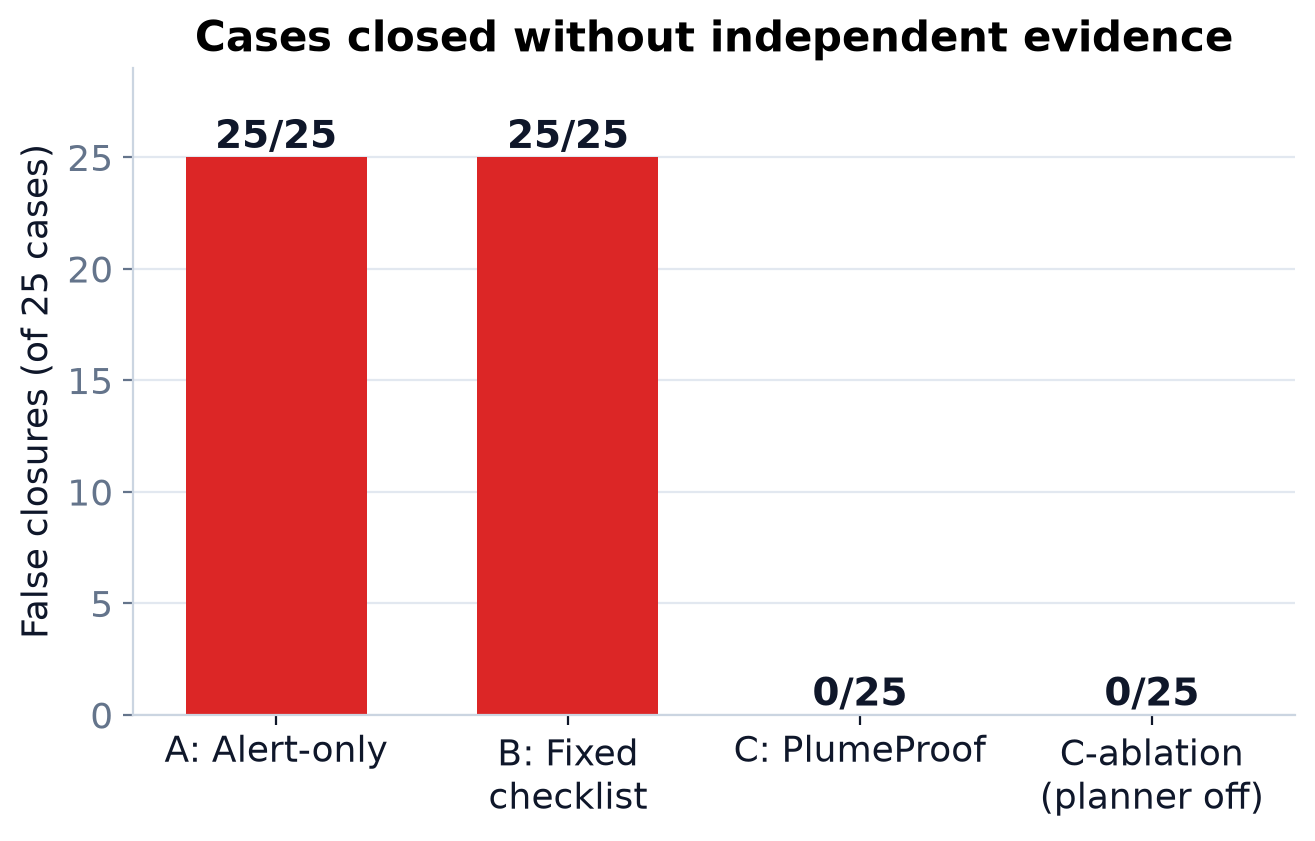
\includegraphics[width=\linewidth]{chart_false_closures.png}
\end{column}
\begin{column}{0.58\textwidth}
\renewcommand{\arraystretch}{1.1}
\scriptsize
\begin{tabular}{@{}l r r >{\columncolor{tealL}}r@{}}
\toprule
& A: Alert-only & B: Checklist & \textbf{C: PlumeProof}\\
\midrule
False closures & {\color{alert}\nFCA} & {\color{alert}\nFCB} & \textbf{\nFCC}\\
Resolved cases & \nResA & \nResB & \textbf{\nResC}\\
Correct source & \nAttrA & \nAttrB & \textbf{\nAttrC}\\
Inspections to find source & \nSrcInspA & \nSrcInspB & \textbf{\nSrcInspC}\\
Cost / resolved case & \nCostAPol & \nCostBPol & \textbf{\nCostCPol}\\
Days to accountable party & \nStakeA & \nStakeB & \textbf{\nStakeC}\\
Decision traceability & \nTraceA & \nTraceB & \textbf{\nTraceC}\\
\bottomrule
\end{tabular}\\[0.2cm]
\card{7.9cm}{\tiny\textbf{Honest reading:} A and B close on the operator's claim, so their closures are false by design. This shows what the evidence gate costs (a verification campaign per case) and that the planner still needs fewer inspections to find the source. All cases simulated.}
\end{column}
\end{columns}
\end{frame}

% =============================== 12. IMPACT / CLOSE ===============================
\begin{frame}{Impact, limits and next steps}
\begin{columns}[T]
\begin{column}{0.31\textwidth}
{\color{teal}\bfseries Impact}\\[3pt]
\scriptsize
\begin{itemize}\setlength\itemsep{3pt}
\item Turns each alert into an owned case with a named accountable party
\item No fix is counted until it is measured
\item Supports the UN goal of an 80\% response rate by 2030 [1]
\item Same design works for coal mines and oil \& gas
\end{itemize}
\end{column}
\begin{column}{0.31\textwidth}
{\color{teal}\bfseries Limits (honest)}\\[3pt]
\scriptsize
\begin{itemize}\setlength\itemsep{3pt}
\item Likelihoods, costs and delays are illustrative
\item Operations and measurements are simulated
\item Bounded measurement noise is assumed
\item Expert review of priorities is not done yet
\end{itemize}
\end{column}
\begin{column}{0.31\textwidth}
{\color{teal}\bfseries Next steps}\\[3pt]
\scriptsize
\begin{itemize}\setlength\itemsep{3pt}
\item Calibrate likelihoods with environmental engineers
\item Pilot with one regulator on real alerts
\item Learn from every closed case (labelled data)
\item PostGIS + task queue for thousands of cases
\end{itemize}
\end{column}
\end{columns}
\vspace*{0.25cm}
\centering

\begin{tikzpicture}\node[draw=teal,line width=1pt,rounded corners=5pt,inner sep=6pt,align=center,text width=12cm]{%
{\large\bfseries Thank you}\\[1pt]
\small Every methane plume deserves an investigation. Every claimed fix deserves evidence.\\[3pt]
\scriptsize\color{slate} github.com/MandarDeshmukh23/RisaavNivaran\ \ ·\ \ 24b4511@iitb.ac.in};\end{tikzpicture}
\end{frame}

% =============================== BACKUP ===============================
\begin{frame}[c]
\centering{\color{teal}\Large\bfseries Backup slides}\\[0.2cm]{\small\color{slate}Assumptions · Tech stack · Sensitivity \& ablation · Scaling · Bayes update · References}
\end{frame}

\begin{frame}{Backup: what is real, what is assumed}
\small
\begin{columns}[T]
\begin{column}{0.48\textwidth}
\REAL\\[3pt]
\begin{itemize}\setlength\itemsep{3pt}
\item Carbon Mapper plumes at Kanjur: 9 Feb 2025 (about 1,600 and 136 kg/h) and 3 Apr 2026 (about 3,300 kg/h combined) [2]
\item Problem statistics from UNEP, IMEO and the literature [1, 4, 5, 7]
\end{itemize}
\vspace*{0.2cm}
\SIM\\[3pt]
\begin{itemize}\setlength\itemsep{3pt}
\item Stakeholder replies, inspector availability, records content, the repair claim and the follow-up measurement
\item All \nNscen{} evaluation scenarios
\end{itemize}
\end{column}
\begin{column}{0.48\textwidth}
{\color{slate}\bfseries ASSUMED (illustrative values)}\\[3pt]
\begin{itemize}\setlength\itemsep{3pt}
\item Prior \nPriorW/\nPriorG/\nPriorF\%, likelihood tables, action costs and durations
\item $\pm$25\% uncertainty on the satellite rate
\item $\lambda$ = \nLambda{} per day
\item Delays: approval 1 day, alert forwarding 30 days, manual stakeholder lookup 7 days, repair 14 days
\item Measurement noise bounded: $|e|\le0.8u$
\item Plume positions inside the site and the wind arrow
\end{itemize}
\end{column}
\end{columns}
\end{frame}

\begin{frame}{Backup: tech stack and budget}
\small
\begin{columns}[T]
\begin{column}{0.55\textwidth}
\renewcommand{\arraystretch}{1.25}
\begin{tabular}{@{}>{\bfseries}l p{5.2cm}@{}}
\toprule
Backend & Python 3.12, FastAPI, Pydantic v2, SQLite\\
Agent & Hand-written orchestrator, 6 tools, approval queue\\
LLM & Optional Claude for drafting; template fallback\\
Frontend & React 18, Vite, Tailwind, Leaflet, Recharts\\
Deploy & One Docker container; Render blueprint\\
Tests & 128 backend tests; 3 browser end-to-end tests\\
\bottomrule
\end{tabular}
\end{column}
\begin{column}{0.4\textwidth}
\card{4.9cm}{\small\textbf{Prototype budget:} about \rupee{}8,000 (about US\$95), from the proposal.\\[4pt]
\scriptsize The core maths takes microseconds per case. The LLM is optional; without a key the app runs fully on templates.\\[4pt]
The ESP32 + MQ-4 demo sensor is uncalibrated and is \textbf{not} used for verification.}
\end{column}
\end{columns}
\end{frame}

\begin{frame}{Backup: sensitivity and ablation}
\begin{columns}[T]
\begin{column}{0.48\textwidth}
\small\textbf{Likelihoods $\pm$20\%} (\nSensDraws{} random draws)
\begin{itemize}\setlength\itemsep{3pt}
\item Top-ranked action unchanged in \textbf{\nSensStab\%} of draws
\item Mean Kendall $\tau$ vs nominal ranking: \textbf{\nSensTau}
\item Agent run on perturbed ``true'' worlds: \textbf{\nSensFC} false closures, \nSensInsp{} inspections per resolved case
\end{itemize}
\vspace*{0.15cm}
\textbf{Planner switched off} (cheapest action first)
\begin{itemize}\setlength\itemsep{3pt}
\item Still \nFCX{} false closures: the gate does its job
\item But \nCloseX{} vs \nCloseC{} days to closure: it starts by waiting 30 days for a satellite pass that carries 0 bits
\end{itemize}
\end{column}
\begin{column}{0.5\textwidth}
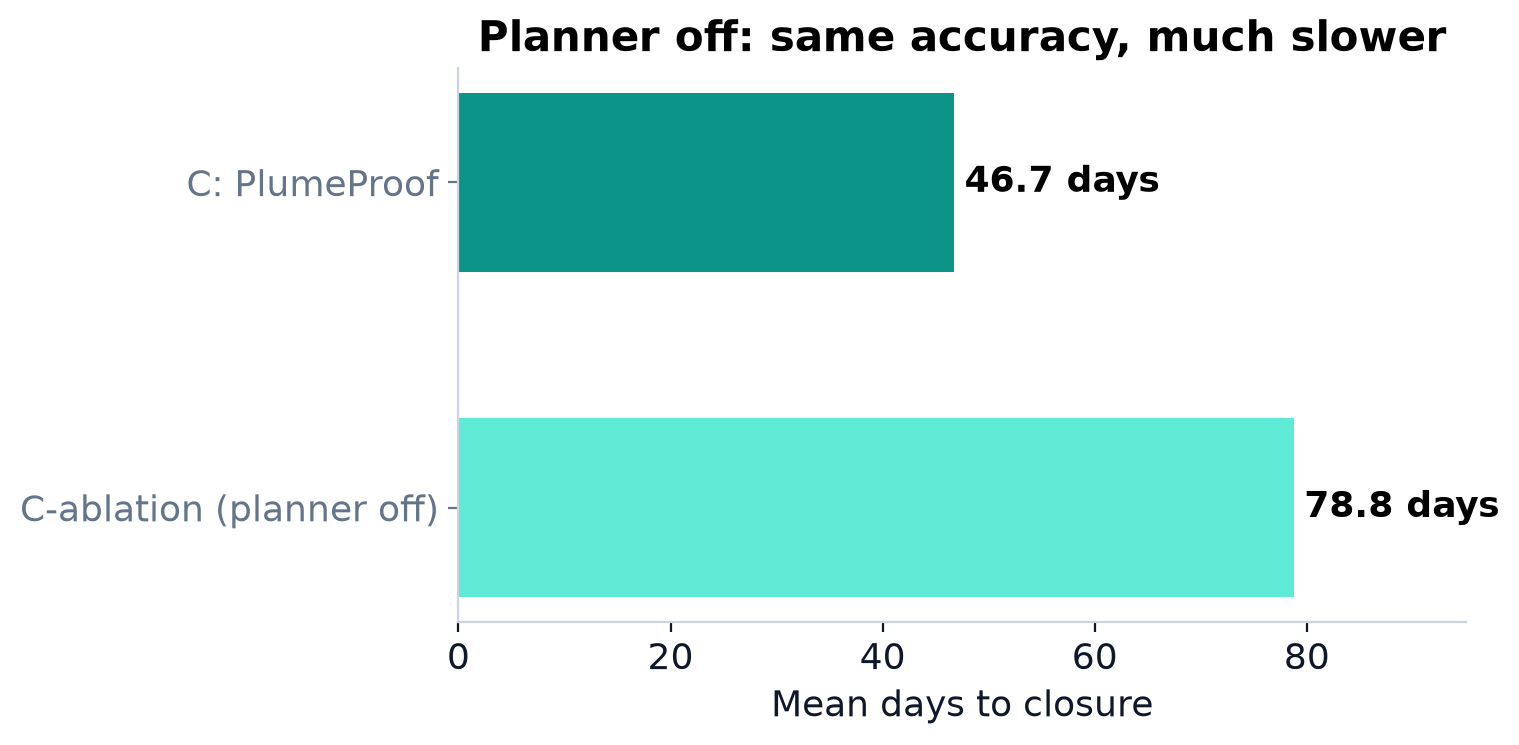
\includegraphics[width=\linewidth]{chart_ablation.png}
\end{column}
\end{columns}
\end{frame}

\begin{frame}{Backup: scaling to 5,000+ alerts}
\small
\begin{columns}[T]
\begin{column}{0.5\textwidth}
\begin{itemize}\setlength\itemsep{5pt}
\item Each case is an independent, small state machine. The maths is microseconds per case.
\item The planner decides \textbf{where scarce human attention goes}: cheap, informative actions first.
\item The approval queue and \texttt{track\_deadline} let a small team supervise many cases; overdue tasks escalate and trigger re-planning.
\item Production path: Postgres/PostGIS, a task queue, regulator-specific jurisdiction tables.
\end{itemize}
\end{column}
\begin{column}{0.47\textwidth}
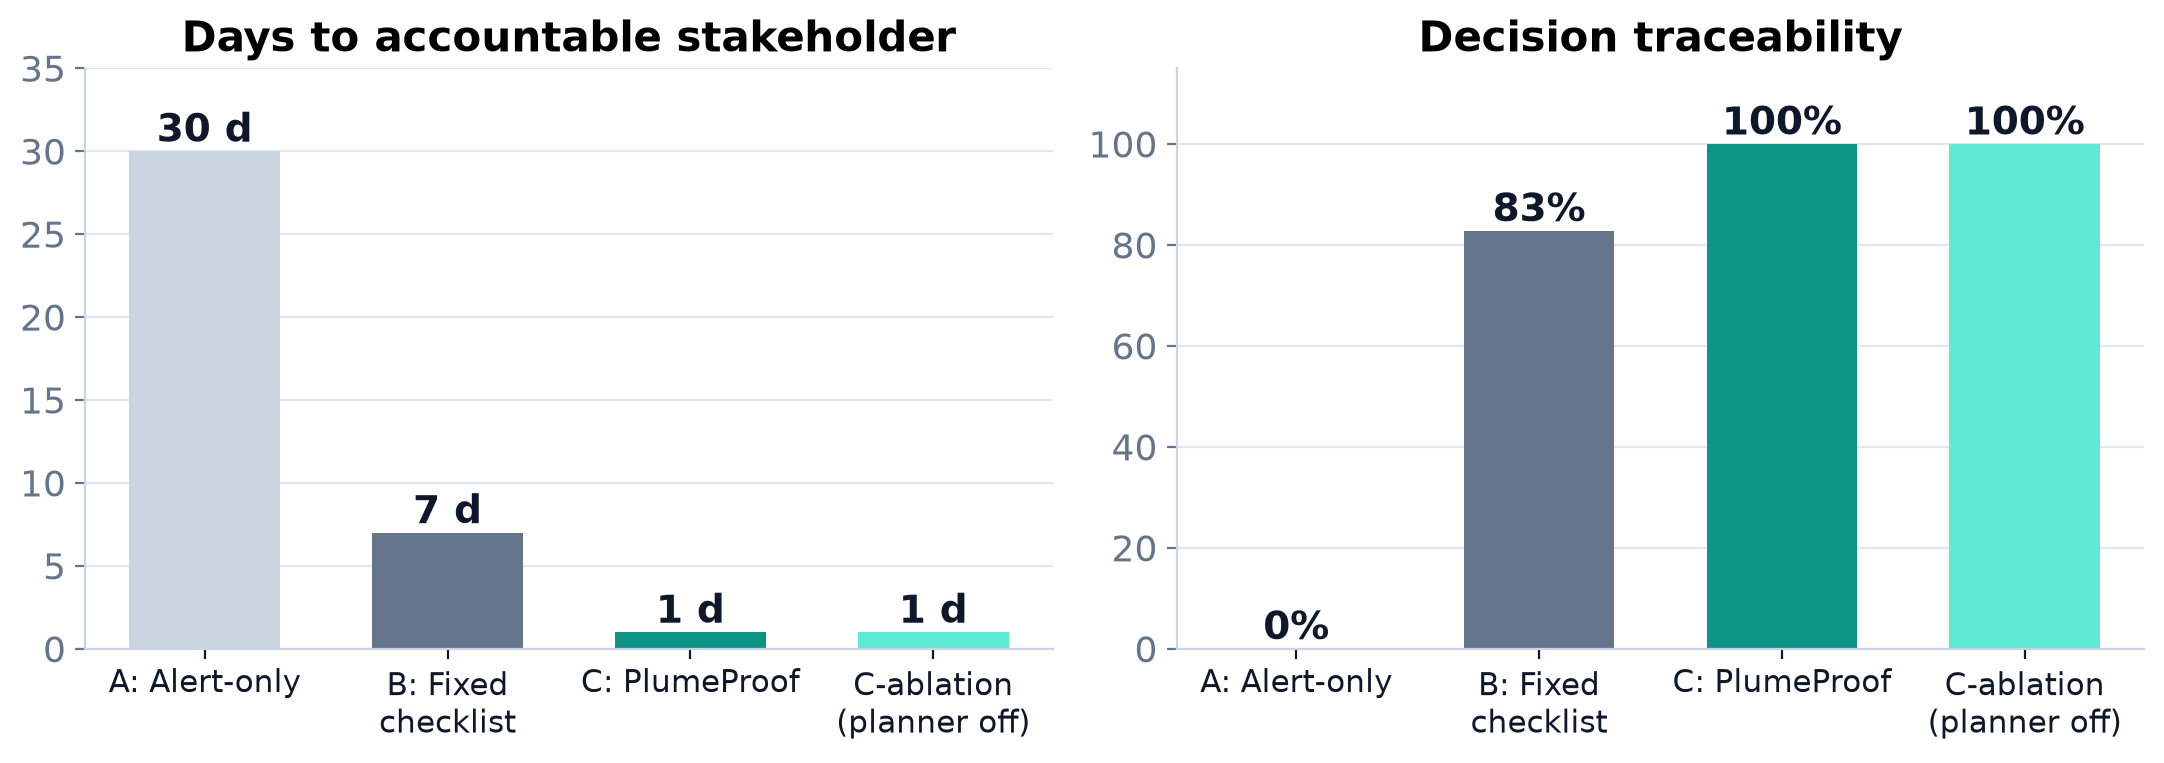
\includegraphics[width=\linewidth]{chart_stakeholder_traceability.png}
\end{column}
\end{columns}
\end{frame}

\begin{frame}{Backup: Bayes update after the records request}
\begin{columns}[T]
\begin{column}{0.52\textwidth}
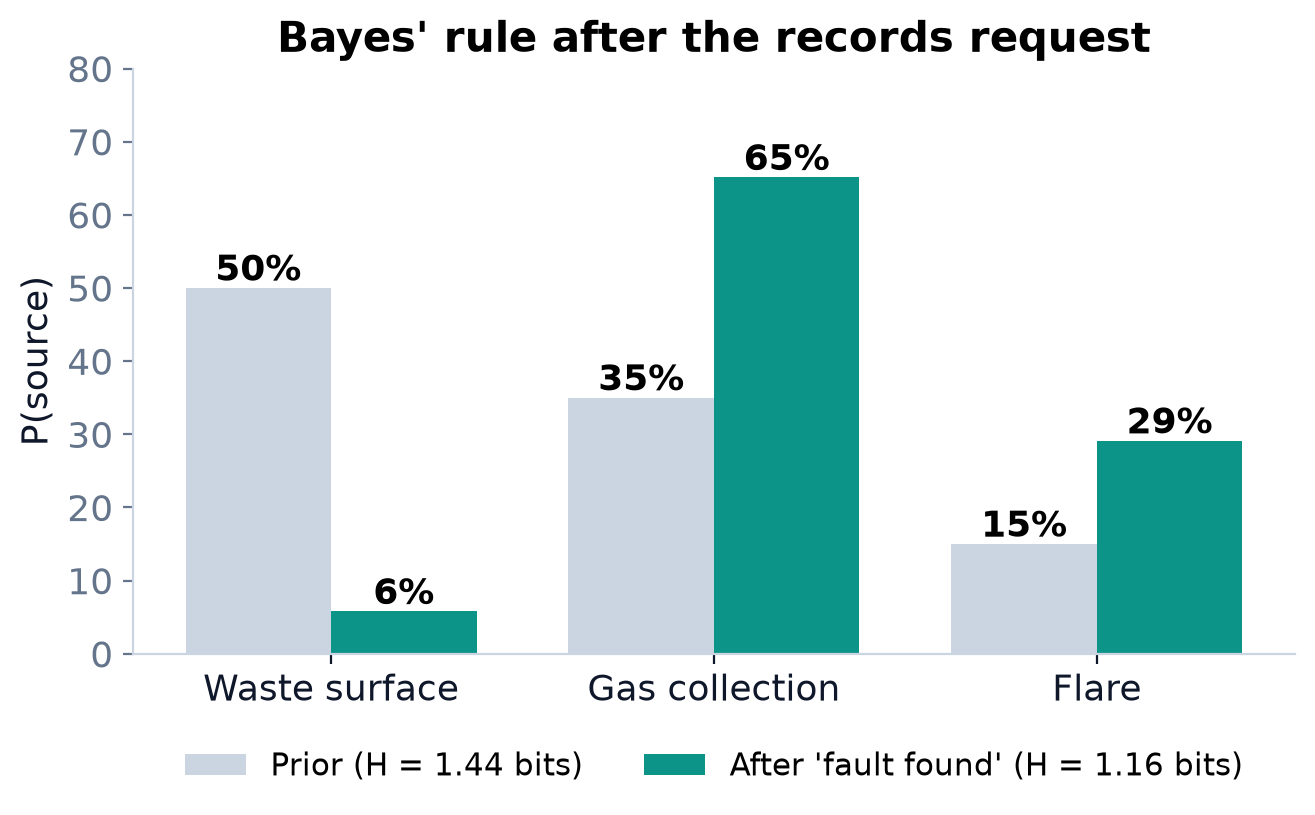
\includegraphics[width=\linewidth]{chart_bayes.png}
\end{column}
\begin{column}{0.45\textwidth}
\small
\[P(h\mid y)\propto P(y\mid h,a)\,P(h)\]
\begin{itemize}\setlength\itemsep{3pt}
\item $P(\text{fault found})=\nPfault$
\item Fault found: gas collection \nPostG\%, flare \nPostF\%, waste \nPostW\%
\item No fault: waste surface \nNoFaultW\%
\item Entropy falls from \nHprior{} to \nHfault{} bits
\end{itemize}
\vspace*{0.1cm}
{\scriptsize\color{slate}Computed live by the engine (What-if page), not typed in. Likelihood values are illustrative.}
\end{column}
\end{columns}
\end{frame}

\begin{frame}{Backup: evidence trail and planner}
\begin{columns}[T]
\begin{column}{0.49\textwidth}\centering
\shot{width=0.985\linewidth}{planner.png}\\[2pt]{\scriptsize Planner: $\lambda$ slider, mark resources unavailable, live re-rank}
\end{column}
\begin{column}{0.49\textwidth}\centering
\shot{width=0.985\linewidth}{audit.png}\\[2pt]{\scriptsize Audit log: every decision linked to its evidence and approver}
\end{column}
\end{columns}
\end{frame}

\begin{frame}{References}
\scriptsize
\begin{enumerate}\setlength\itemsep{4pt}
\item[{[1]}] UNEP (23 June 2026). UNEP, partners ramp up efforts to address major methane leaks as UN chief urges rapid cuts. Press release.
\item[{[2]}] Carbon Mapper (22 July 2026). Examining methane emissions at Mumbai waste sites. carbonmapper.org/articles/mumbai-waste-sites
\item[{[3]}] Down To Earth (5 May 2026). UN methane alert system expanded to coal and waste sectors after Indian landfill named among world's top emitters.
\item[{[4]}] UNEP IMEO (May 2026). Mapping the world's biggest methane sources and tracking country response: MARS snapshot.
\item[{[5]}] Allen, A., Mateo-Garcia, G., et al. (2025). Artificial intelligence for methane detection: from continuous monitoring to verified mitigation. arXiv:2511.21777
\item[{[6]}] NASA/JPL-Caltech (2022). EMIT methane plume image, PIA25592.
\item[{[7]}] IISD SDG Knowledge Hub (2025). UN report calls for scaling action on methane through data-driven solutions.
\end{enumerate}
\end{frame}

\end{document}
